\documentclass{standalone}
\usepackage{tikz}
\usepackage{ctex,siunitx}
\usepackage{tkz-euclide}
\usepackage{amsmath}
\usetikzlibrary{patterns, calc}
\usetikzlibrary {decorations.pathmorphing, decorations.pathreplacing, decorations.shapes,}
\begin{document}
\small
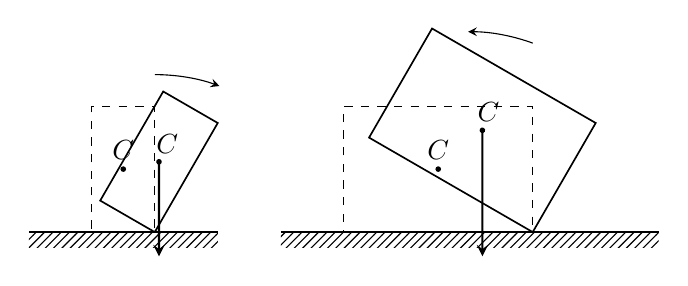
\begin{tikzpicture}[>=stealth,scale=0.8]
  \fill [pattern=north east lines](-2,-.25) rectangle (1,0);
  \draw [thick](-2,0)--(1,0);
  \draw [dashed] (0,0)--(-1,0)--(-1,2)--(0,2)--(0,0);
  \draw[rotate=-30,semithick] (0,0)--(-1,0)--(-1,2)--(0,2)--(0,0);
  \draw[fill=black] (-.5, 2/2) circle (1pt); 
  \draw[fill=black,rotate=-30] (-.5, 2/2) circle (1pt); 
  \draw [->, thick, rotate=-30](-.5, 2/2)--+(-60:1.5);
  \draw[->] (0,2.5) arc (90:70: 3);
  \node at (-.5, 2/2)[above]{$C$};
  \node at (0.2, 2/2+.1)[above]{$C$};
  \begin{scope}[xshift=6cm]
    \fill [pattern=north east lines](-4,-.25) rectangle (2,0);
    \draw [thick](-4,0)--(2,0);
    \draw [dashed] (0,0)--(-3,0)--(-3,2)--(0,2)--(0,0);
    \draw[rotate=-30,semithick] (0,0)--(-3,0)--(-3,2)--(0,2)--(0,0);
    \draw[fill=black] (-1.5, 2/2) circle (1pt); 
    \draw[fill=black,rotate=-30] (-1.5, 2/2) circle (1pt); 
    \draw [->, thick, rotate=-30](-1.5, 2/2)--+(-60:2);
    \draw[->] (0,3) arc (70:90: 3);
    \node at (-1.5, 2/2)[above]{$C$};
    \node at (-.7, 2/2+.6)[above]{$C$};
  \end{scope}
\end{tikzpicture}
\end{document}